\documentclass{beamer}
\usetheme{metropolis}
\usepackage{graphicx}
\usepackage{amsmath}
\title{Digital Signal Processing: COSC390}
\author{Jordan Hanson}
\institute{Whittier College Department of Physics and Astronomy}

\begin{document}
\maketitle

\begin{frame}{Quiz 1}
Suppose the following symbol represents an LTI system that delays the input signal by $n$ samples:
\begin{figure}
\centering
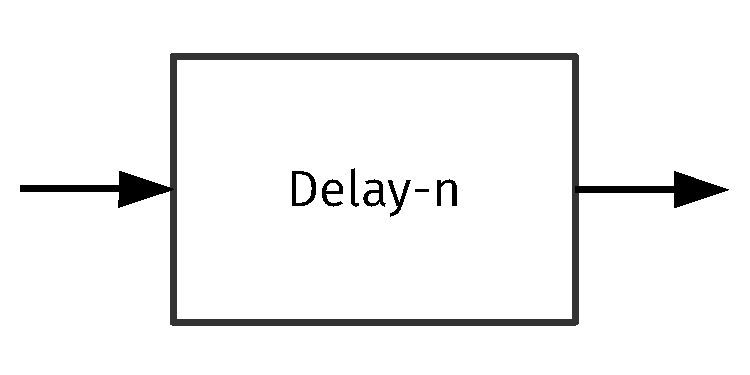
\includegraphics[width=0.3\textwidth]{delay-n.pdf}
\caption{\label{fig:n} An LTI system that delays the input by $n$ samples.}
\end{figure}
\end{frame}

\begin{frame}{Quiz 1}
\small
Write or graph the transfer function $r[n]$, that represents $z[n] = r[n] \circ x[n]$:
\begin{figure}
\centering
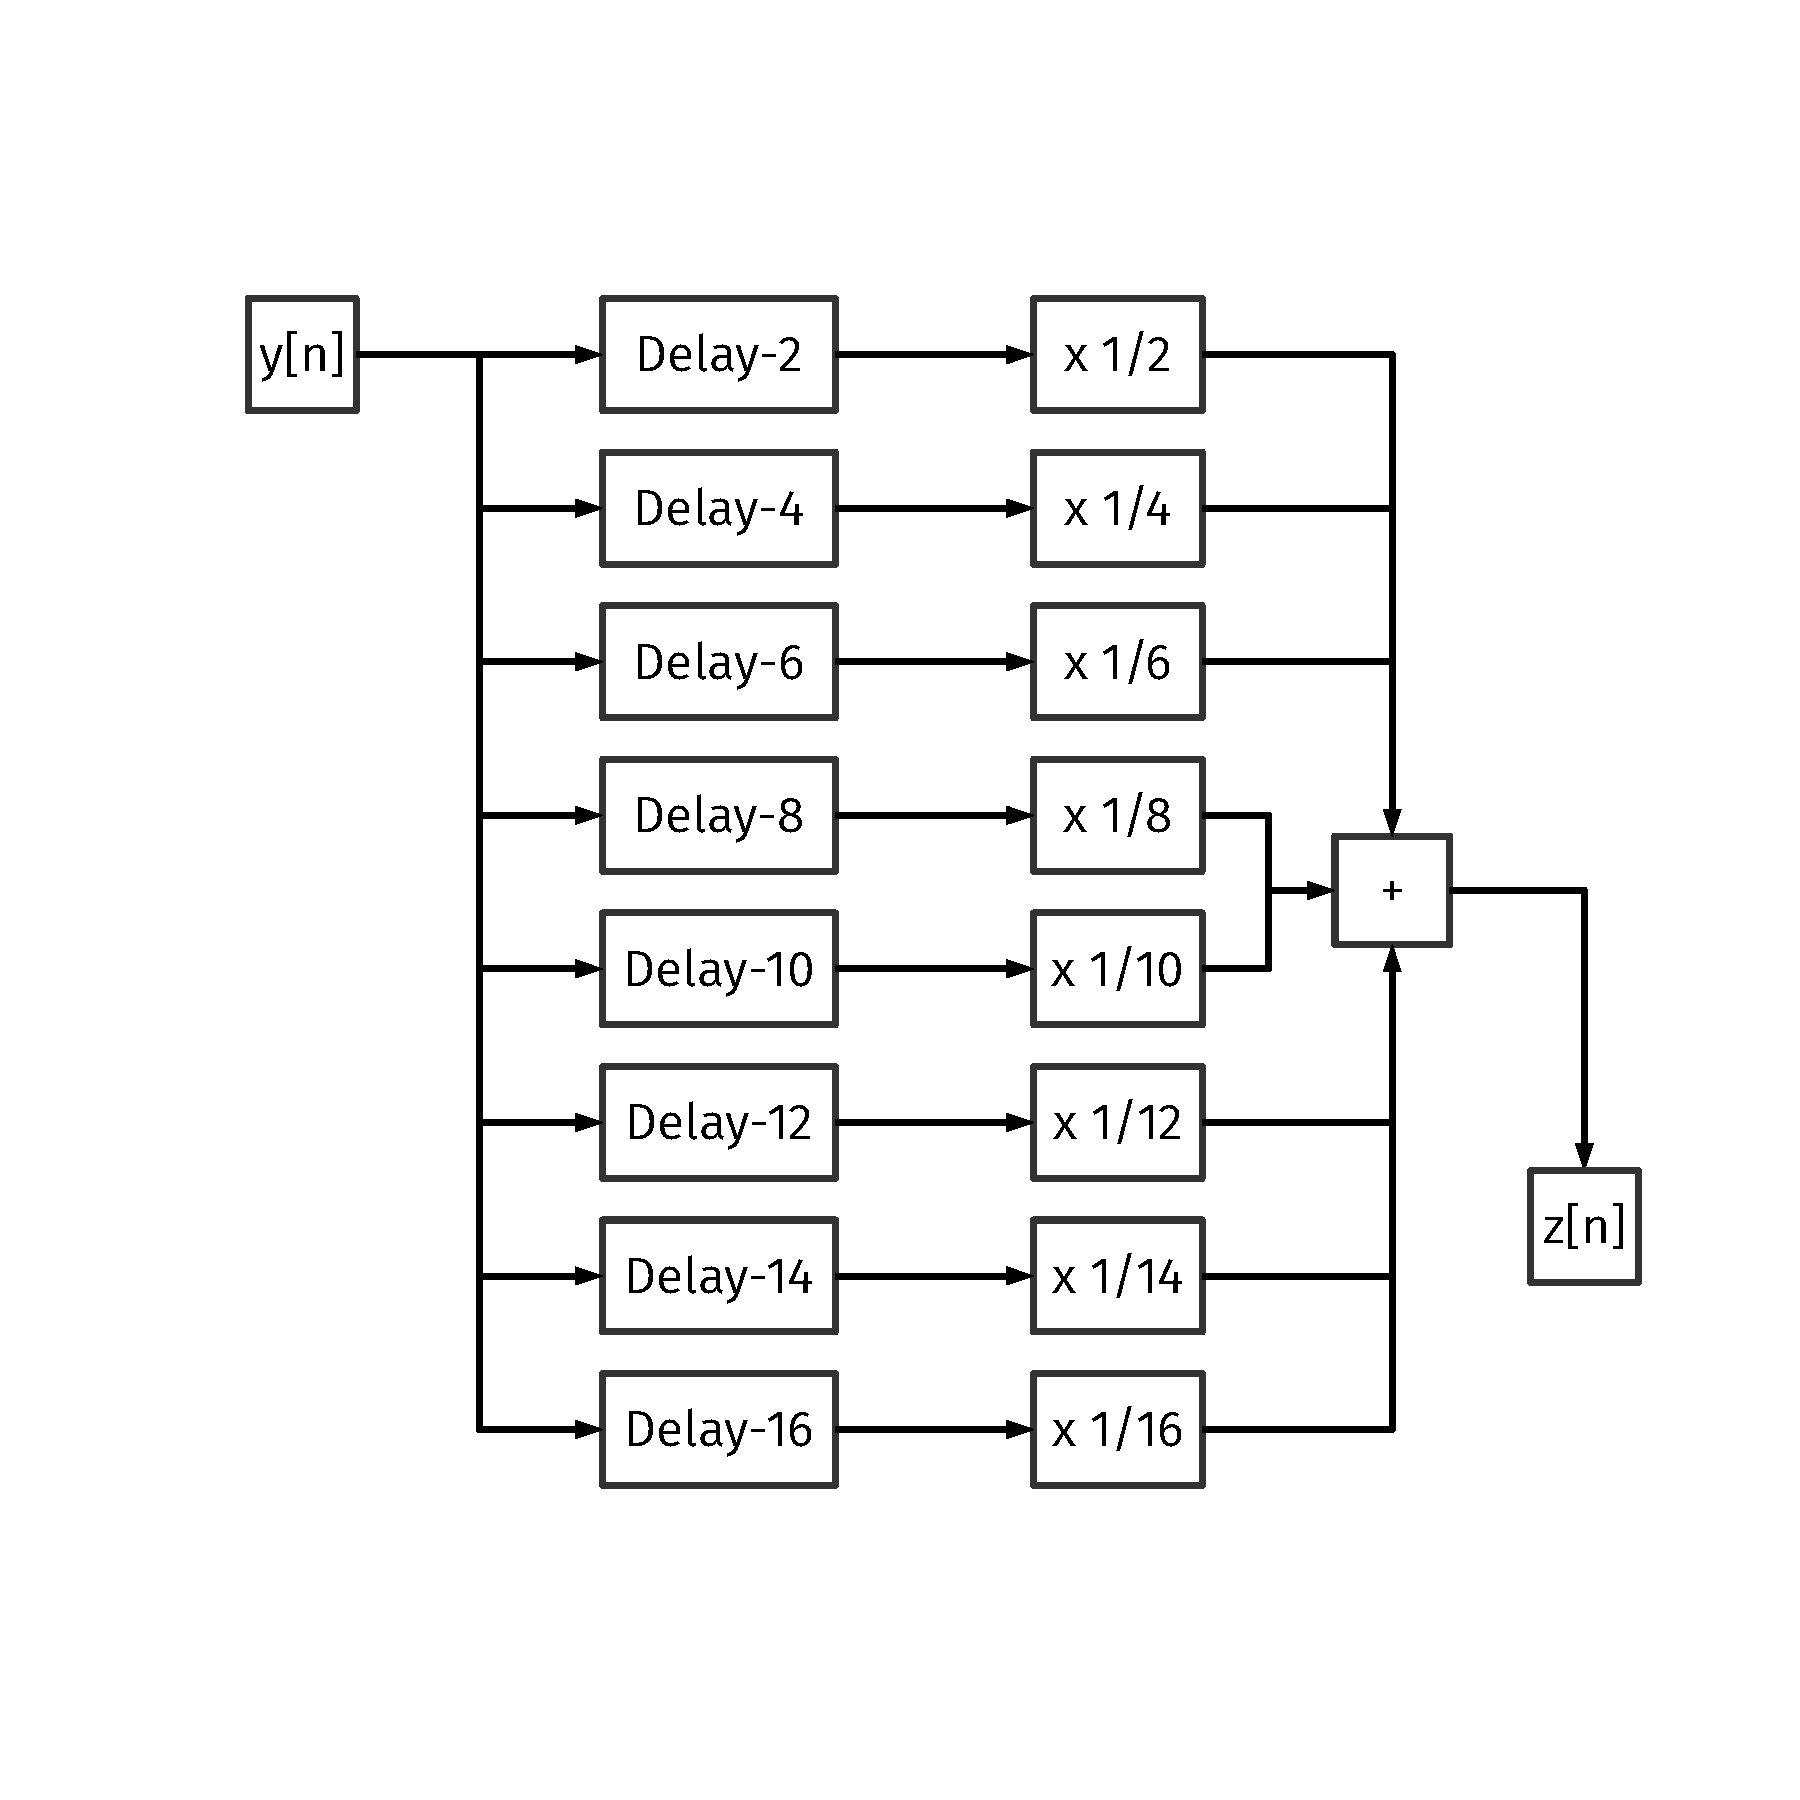
\includegraphics[width=0.6\textwidth,trim=2cm 4cm 2cm 4cm,clip=true]{delay-sum.pdf}
\caption{\label{fig:nsum} A combination of LTI systems.}
\end{figure}
\end{frame}

\end{document}